\section{Definitions of the Constants, Costs, Variables and Functions}
This section is more intended for mathematicians and computer scientists too. Those who don't wish to read the mathematical parts should still broadly understand the variables of harmonic intervals, melodic intervals and motions (\textbf{H}, \textbf{M} and \textbf{P} in section \ref{sec:variables}). Subsections \ref{sec:constants} and \ref{sec:variables} describes the various names used in the mathematical parts and in the Lisp code of the solver (immediately to their right, e.g. \textbf{n} \space \texttt{*total-cp-len}). These subsections explain also how those constants and variables work. Unless otherwise stated, all domains of constants and variables belong to the domain of integers $\mathbb{N}$.

% CONSTANTS
\subsection{Constants}\label{sec:constants}
Constants are only constant with respect to the Gecode solver, so they are deduced before a solution is sought by the latter.

\paragraph{Cons $_{(all,\ p,\ imp)}$} \texttt{ALL\_CONS}, \texttt{P\_CONS}, \texttt{IMP\_CONS}

Set representing all consonances, perfect consonances and imperfect consonances respectively. By default, the notation $Cons \equiv Cons_{all}$.

\begin{equation}
    \begin{gathered}
        Cons_{p} := \{0, 7\}\\
        Cons_{imp} := \{3, 4, 8, 9\}\\
        Cons_{all} := Cons_{p} \cup Cons_{imp} \equiv \{0, 3, 4, 7, 8, 9\}
    \end{gathered}
\end{equation}

\paragraph{species} \texttt{species}

Chosen species of counterpoint. $species \in \{1, 2, 3, 4, 5\}$.

\paragraph{m} \texttt{*cf-len}

Number of measures which is equivalent to the number of notes in the \cfdot $m \in [3, 17]$. $3$ because the solver needs al least 3 measures to work properly. $17$ is arbitrary and comes from $4\times 4 + 1$, i.e. a commun number of measure $\times$ a number not too large for the computation $+$ one final measure.

\paragraph{n} \texttt{*total-cp-len}

Number of notes in the counterpoint depending on the chosen species. $n \in [1, b(m-1)+1]$ because the last measure has necessarily a whole note.

\paragraph{s$_{m}$}

Maximum number of notes contained in the counterpoint, all species combined, i.e. if the counterpoint contained only quarter notes, with the exception of the last note being a whole note.

\begin{equation}
    s_{m} = m + 3\times (m-1) \text{ and }s_{m-1} = (m-1) + 3\times (m-2)
\end{equation}

Used as the size for an array containing one list of size $m$ (or $m-1$) the notes in thesis and three lists of size $m-1$ (or $m-2$) the other beats. The difference with $n$ is that $s$ does not depend on $b$.

\paragraph{Cf} \texttt{*cf}

List of size $m$ representing the MIDI notes of the \cfdot

\begin{equation}
    \begin{gathered}
        \forall j \in [0, m)\\
        Cf[j] \in [0, 127]
    \end{gathered}
\end{equation}

\paragraph{M$_{cf}$} \texttt{*cf-brut-m-intervals}

List of size $m-1$ representing the melodic intervals between the consecutive notes of the \cfdot

\begin{equation}
    \begin{gathered}
        \forj\\
        M_{cf}[j]=Cf[j+1]-Cf[j]\\
        \text{where } M_{cf} \in [-127, 127]
    \end{gathered}
\end{equation}
% N.B.: any melodic interval should ideally be in the range $[-12, 12]$.

\paragraph{lb} \texttt{RANGE\_LB}

Lower bound of the range of the notes of the counterpoint. $lb \in [0, ub)$.

\paragraph{ub} \texttt{RANGE\_UB}

Upper bound of the range of the notes of the counterpoint. $ub \in (lb, 127]$.

\paragraph{$\R$} \texttt{*cp-range}

Range of the notes of the counterpoint. $\R := [lb, ub]$.

\paragraph{borrow} \df{major}\footnote{\df{value} means the default value in the tool.}

Determines the "borrowing scale", i.e. the additional notes that the counterpoint can have in relation to the tonic of the piece. More details will be given on what are the borrowed notes in section \ref{sec:generalenglish}.

\begin{equation}
    \begin{gathered}
        borrow \in \{none, major, minor\}
    \end{gathered}
\end{equation}

\paragraph{$\N_{(all,\ key,\ brw)}^{(\R)}$} \texttt{*extended-cp-domain}, \texttt{*scale}, \texttt{*borrowed-scale}.

Set of values available for the notes of the counterpoint. $\N_{key}$ represents the notes of the key provided by the user's score. $\N_{brw}$ represents the additional borrowed notes that the counterpoint can have in relation to the tonic of the piece. $\N_{all}$ represents the union of the two previous sets. If $borrow = none$ then $\N_{brw} = \emptyset$ and $\N_{all} = \N_{key}$. $\N_{(all,\ key,\ brw)}^{\R}$ represents the set of notes bounded to the range, i.e. the intersection of $\N_{(all,\ key,\ brw)}$ and $\R$. By default, $\N$ refers to $\N_{all}$ not bounded to the range.

\begin{equation}
    \begin{gathered}
        \N_{key} := buildScale(key, scale)\\
        \N_{brw} := \begin{cases}
            \emptyset & \text{if } borrow = none\\
            buildScale(Cf[0]\ mod\ 12, "borrowed") & \text{if } borrow = major\\
            buildScale([Cf[0]+3]\ mod\ 12, "borrowed") & \text{if } borrow = minor
        \end{cases}\\
        \N_{all} := \N_{key} \cup \N_{brw}\\
        \N_{(all,\ key,\ brw)}^{\R} := \N_{(all,\ key,\ brw)} \cap \R\\
    \end{gathered}
\end{equation}

Where $buildScale(key, scale)$ (see function \ref{eq:buildScale}) is a function that returns the set of notes in the $key$ based on the $scale$ used. Also more details on the borrowed notes will be given in section \ref{sec:generalenglish}.

\subsection{Costs}
The costs are constants chosen by the user that have default values supposed to represent Fux's preferences.

\paragraph{pref and cost} \texttt{*params*}

A preference can have 7 levels of intensity ranging from "no cost" to "forbidden". For any cost $cost$ and any preference $pref$, it can be defined that:

\begin{equation}
    \begin{gathered}
        cost = \begin{cases}
            0 & \text{if } pref = \text{no cost}\\
            1 & \text{if } pref = \text{low cost}\\
            2 & \text{if } pref = \text{medium cost}\\
            4 & \text{if } pref = \text{high cost}\\
            8 & \text{if } pref = \text{last resort}\\
            2m & \text{if } pref = \text{cost prop. to length}\\
            64m & \text{if } pref = \text{forbidden}
        \end{cases}
    \end{gathered}
\end{equation}

$64m$ is a ridiculously huge value that will never be reached by all the other costs combined even if they were all high.

\paragraph{Cond$_{costs}$ and cost$_{Cond}$} All costs work the same way: a list of boolean variables, called $Cond$ for the explanation, determines whether it is true that a certain cost should be established for this specific condition in certain locations. The list of assigned costs for this condition is noted $Cond_{costs}$. The elements of $Cond_{costs}$ are thus equivalent to any cost $cost$ depending on the preference $pref$ chosen for the condition $Cond$. The different costs for the different types of conditions each have their own identifier noted $cost_{Cond}$. It is this value that changes depending on the user's preference. To sum up:

% \begin{equation}
%     \begin{gathered}
%         \forall c \in Cond_{costs}, \forall cond \in Cond\\
%         c = \begin{cases}
%             cost_{Cond} & \text{if } cond \text{ is true}\\
%             0 & \text{otherwise}
%         \end{cases}\\
%         \text{where } cost_{Cond} \in dom(cost)
%     \end{gathered}
% \end{equation}

\begin{equation}
    \begin{gathered}
        \forall \rho \in Positions(Cond)\\
        Cond_{costs}[\rho] = \begin{cases}
            cost_{Cond} & \text{if } Cond[\rho] \text{ is true}\\
            0 & \text{otherwise}
        \end{cases}\\
        \text{where } Positions(Cond) \text{ is the set of positions where the condition } Cond \text{ applies}\\
        \text{ and where } cost_{Cond} \in dom(cost)
    \end{gathered}
\end{equation}

\paragraph{$\C$ and $\tau$} \texttt{*cost-factors}, \texttt{*total-cost}.

The heuristic of the solver leads to find a solution while minimizing the total cost. The latter is represented by $\tau$ while $\C$ is a set of integers representing all the sums of the different lists of costs. $\tau$ is thus the sum of all the elements of $\C$. If $Costs$ is the set of all the different $Cond_{costs}$ lists then:

\begin{equation}
    \begin{gathered}
        \C = \bigcup _{\forall \chi \in Costs} \ \sum _{\forall c \in \chi} c\\
        \tau := \sum _{\forall \sigma \in \C} \sigma\\
        \min \tau
    \end{gathered}
\end{equation}

By definition, for any forbidden $pref$ to be indeed \emph{forbidden}, the following constraint must be added:

\begin{equation}
    \begin{gathered}
        \sum _{\forall \sigma \in \C} \sigma < 64m
    \end{gathered}
\end{equation}

% VARIABLES
\subsection{Variables}\label{sec:variables}
Variables are fully deduced by the Gecode solver and their values can be evaluated only after a solution has been found.

Many variables have a general definition so that they can be used in all equations, this does not mean that all possible combinations have been defined in the Lisp code but only those that are actually used. For example, there is no need to have access to all possible melodic intervals in the solver, however the mathematical notation would allow it.

If some letters are not defined, it means that they have already been defined in the constants or in the previous variables.
\paragraph{Cp} \texttt{*cp} %%% COUNTERTPOINT %%%

Array of size $s_{m}$ representing the MIDI notes of the counterpoint. This array is thus composed of four lists, each representing a beat on all the measures of the song. As explained above, this is how all the other arrays related to the countrepoint (i.e. the $Cp$ array) are constructed.

For example, for a whole notes counterpoint: the relevant $Cp$ would be only the list $Cp[0]$. For a half notes counterpoint: it would be the merge of $Cp[0]$ and $Cp[2]$. For a quarter notes counterpoint: it would be the merge of $Cp[0]$, $Cp[1]$, $Cp[2]$ and $Cp[3]$.

\begin{equation}
    \forall i \in \B, \forall j \in [0, m): Cp[i, j]\in \N^{\R}
\end{equation}

Figure \ref{fig:solverdiagram} shows a popularization of the tool's logic vis-à-vis these arrays of variables.

\begin{figure}
    \centering
    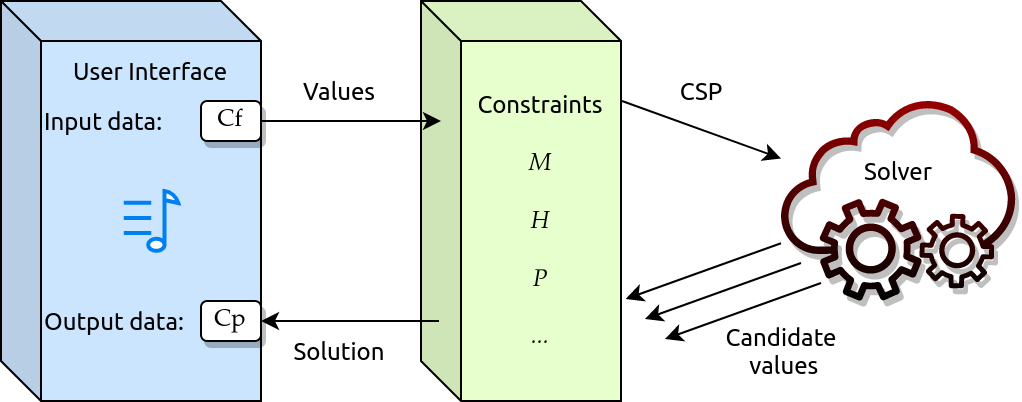
\includegraphics[height=1.7in]{Images/solver_diagram.png}
    \caption{Popularization of the tool's logic vis-à-vis the arrays of variables.}
    \label{fig:solverdiagram}
\end{figure}

\paragraph{H$_{(abs)}$} \texttt{*h-intervals, *h-intervals-abs.} %%% HARMONIC INTERVALS %%%

Array of size $s_{m}$ representing each harmonic interval between the counterpoint and the \cfdot There are four lists of harmonic intervals, each representing a beat along the whole counterpoint. The harmonic intervals are calculated so that they represent the absolute difference between the pitch of the counterpoint and the pitch of the \cfdot Since the values are absolute, it does not matter if the \cf is lower or upper, the intervals will always be calculated according to the lowest note. Any harmonic interval is calculated according to the notes played at the same time in the \cf and the counterpoint. Therefore, up to four notes in the counterpoint can be calculated with respect to the same note in the \cfdot

Two versions of that array-variable exist: the main one $H$ which is modulo 12 and $H_{abs}$ which is not. It is always true that $H = H_{abs}\ mod\ 12$. Unless mentioned, when talking about "harmonic intervals" or "harmonies", it refers to the variables of the array $H$.

\begin{equation}
    \begin{gathered}
        \forall i \in \B, \forall j \in [0, m)\\
        H_{abs}[i, j] = \left|Cp[i, j] - Cf[j]\right|\\
        H[i, j] = H_{abs}[i, j]\ mod\ 12\\
        \text{where } H_{abs}[i, j] \in [0, 127], H[i, j] \in [0, 11]
    \end{gathered}
\end{equation}

$12$ representing the number of semitones in an octave. This allows the interval between a note and any note higher at different octaves to always be the same. This implies that $H \in$ table \ref{tab:intervalsvalues} values. For example, for the gap between $C_4$ (60) and $G_4$ (67) and the gap between $C_4$ (60) and $G_5$ (79), the $H_{abs}$ values will be 7 and 19 while the $H$ values will be 7 and 7.

\begin{figure}[h]
    \centering
    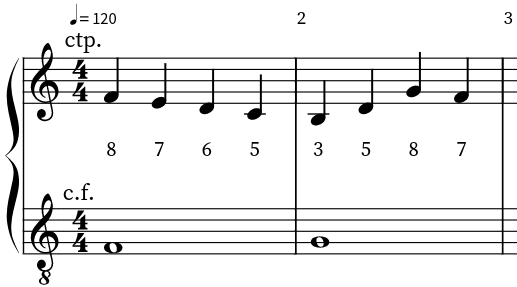
\includegraphics[width=2.5in]{Images/harmonic_intervals_variables.png}
    \caption{Traditionally written harmonies between the ctp. and the \cfdot}
    \label{fig:harmonicintervals}
\end{figure}

Beware that the numbers noted on figure \ref{fig:harmonicintervals} are those used on scores. They refer to the names of the intervals and not to the relative MIDI values. By contrast, table \ref{tab:hjarrayvar} below shows the MIDI values of the intervals for this figure.

\begin{table}[h]
    \centering
    \begin{tabular}{|c||c|c|c|c|}
    \hline
    measure $j$ & $H_{abs}[0, j]$ & $H_{abs}[1, j]$ & $H_{abs}[2, j]$ & $H_{abs}[3, j]$ \\ \hline
    0 & 12 & 11 & 9 & 7 \\ \hline
    1 & 4 & 7 & 12 & 10 \\ \hline
    \end{tabular}
    \caption{Relative MIDI values of figure \ref{fig:harmonicintervals}.}
    \label{tab:hjarrayvar}
\end{table}

\paragraph{M$^{(x)}_{(brut)}$} %%% MELODIC INTERVALS %%%

\texttt{*m-intervals, *m-intervals-brut, *m2-intervals, \dots}
%  *m2-intervals-brut,\\
% *m-succ-intervals, *m-succ-intervals-brut.}

Arrays of size $s_{m-x}$ representing each melodic interval between a note of the counterpoint at a specific beat and another further note of the counterpoint at another specific beat. The melodic intervals are calculated so that they represent the difference between the two notes involved.

The array is noted $M^x$ where $x$ is the number of $d$\footnote{Duration of a note in beat(s) depending on the chosen species (see $d$ in above section \ref{sec:constants}).} beat(s) that separates the initial note to the further one. $x$ represents the desired number of notes between the current note and the one of interest to calculate the melodic interval. In other words, $M^x[i, j]$ represents the melodic interval between the note at beat $i$ in measure $j$ and the note at beat $[(i+xd)\ mod\ 4]$ in measure $[j+nextm(i+xd)]$. If $x$ is not present then its default is 1. For example, with whole notes (i.e. $d=4$): $M[0, 5]$ represents the melodic interval between the note in the sixth measure ($j=5$) and the note in the seventh measure ($j=6$).

There are two versions of that array-variable: the main one $M^x$ which is absolute and $M^x_{brut}$ which is not. It is always true that $M^x = \left|M^x_{brut}\right|$. Unless mentioned, when talking about "melodic intervals" or "melodies", it refers to the variables of the array $M^1$. See figure \ref{fig:threetypesofnotes} (the corresponding midi value is annotated below each note) and table \ref{tab:mxarrayvar} for clarity.
\begin{equation}
    \begin{gathered}
        \forall x \in \{1, 2\}, \forall i \in \B, \forall j \in [0, m-x)\\
        M^x_{brut}[i, j] = Cp[(i+xd)\ mod\ 4, j+nextm(i+xd)] - Cp[i, j]\\
        M^x[i, j] = \left|M^x_{brut}[i, j]\right|\\
        \text{where } M^x_{brut}[i, j] \in [-12, 12], M^x[i, j] \in [0, 12]
    \end{gathered}
\end{equation}

The intervals are limited to $12$ because the octave leap is the maximum that can be reached.

\begin{figure}[h]
    \centering
    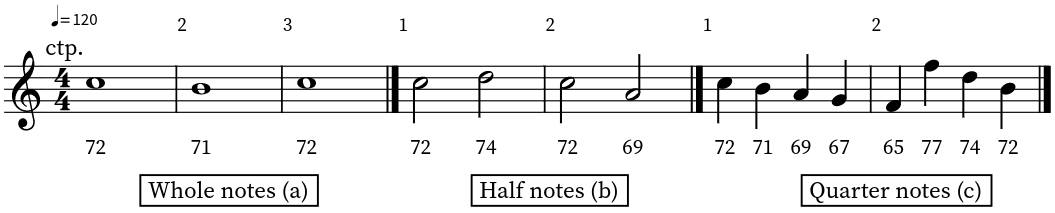
\includegraphics[height=1in]{Images/melodic_intervals_variables.png}
    \caption{The 3 types of notes that can be used in the counterpoint.}
    \label{fig:threetypesofnotes}
\end{figure}

\begin{table}[h]
    \centering
    \begin{tabular}{|c|||c||c||c|}
    \hline
    $M^x_{(brut)}$      & Whole notes (a) & Half notes (b) & Quarter notes (c) \\ \hline \hline
    $M[0, 0]$   & 1 (-1)        & 2 (2)          & 1 (-1)            \\ \hline
    $M[1, 0]$   & $\emptyset$   & $\emptyset$    & 2 (-2)            \\ \hline
    $M[2, 0]$   & $\emptyset$   & 2 (-2)         & 2 (-2)            \\ \hline
    $M[3, 0]$   & $\emptyset$   & $\emptyset$    & 2 (-2)            \\ \hline
    $M[0, 1]$   & 1 (1)         & 3 (-3)         & 12 (12)            \\ \hline
    $M^2[0, 0]$ & (0)           & 0 (0)          & 3 (-3)            \\ \hline
    $M^2[2, 0]$ & $\emptyset$   & 5 (-5)         & 4 (-4)            \\ \hline
    \end{tabular}
    \caption{Some relative MIDI values of figure \ref{fig:threetypesofnotes} with $x=\{1, 2\}$.}
    \label{tab:mxarrayvar}
\end{table}

In the solver, melodic intervals used are stored in several lists by beat pair, e.g. one list for all the intervals between the first and second beats of all measures. The constraints to represent these calculations are done separately from one table to another with the same function. From example, all the melodic intervals between the fourth beat note and the next first beat note in the thrid species are computed like in equation \ref{eq:melo30example}:

\begin{equation}
    \begin{gathered}
        \forj\\
        M_{brut}[3, j] = Cp[0, j+1] - Cp[3, j]\\
        M[3, j] = \left|M_{brut}[3, j]\right|\\
    \end{gathered}
    \label{eq:melo30example}
\end{equation}

\paragraph{P} \texttt{*motions} %%% MOTIONS %%%

Array of size $4\times (m-1)$ representing each motion between two consecutive measures. The letter $P$ is for \textit{passage} since $M$ is already taken.
% The motions are calculated in such a way that they directly represent the cost of themselves. By default, contrary motions are the most appreciated and have no cost. Oblique motions are not restricted and have a cost of 1. Direct motions are less appreciated and have a cost of 2.
Contrary, oblique and direct motions are represented by 0, 1 and 2 respectively.

\begin{equation}
    \begin{gathered}
        \forall x \in \{1, 2\}, \forall i \in \B, \forj, x := b-i\\
        P[i, j] =
        \begin{cases}
            0 & \text{if } (M^{x}_{brut}[i, j] > 0 > M_{cf}[j]) \lor (M^{x}_{brut}[i, j] < 0 < M_{cf}[j]) \\
            1 & \text{if } M^{x}_{brut}[i, j] = 0 \lor M_{cf}[j] = 0 \\
            2 & \text{if } (M^{x}_{brut}[i, j] > 0 \land M_{cf}[j] > 0) \lor (M^{x}_{brut}[i, j] < 0 \land M_{cf}[j] < 0)
        \end{cases}
        % \text{where } P[i, j] \in \{0, 1, 2\}
    \end{gathered}
\end{equation}

$x:=b-i$ represents the fact that the motion is obtained between the current note and the first note of the next measure. For example, with quarter notes, the gap between the third note and the first note of the next measure is defined as: $b=4$, $i=2$ and $x=4-2=2$. The first note of the next measure is therefore 2 notes away.

The motions require relatively many constraints to be computed. Indeed, a boolean variable is needed for each type of direction of the counterpoint melody (3) as well as that of the \cf (3). This gives 3*3 different possibilities to be divided into 3 categories of motions for each measure. This is not a problem in itself but with GiL, any boolean operation must be computed via a constrained boolean variable. Ideally one should use argument variables provided by Gecode that are intended to be temporary variables. Implementing this in GiL would probably improve performance.

\paragraph{IsCfB} \texttt{*is-cf-bass-arr}

Boolean array of size $s_{m}$ representing if the \cf is below. Each list of this array represents a beat along the whole counterpoint and is calculated by comparing the pitch of the counterpoint with the pitch of the \cf at the same time.

\begin{equation}
    \begin{gathered}
    \forall i \in \B, \forall j \in [0, m)\\
    IsCfB[i, j] =
    \begin{cases}
        \top & \text{if } Cp[i, j] \geq Cf[j] \\
        \bot & \text{otherwise}
    \end{cases}
    \end{gathered}
\end{equation}

By default, if both notes are the same then the \cf is considered as the bass.

\paragraph{IsCons$_{(all,\ p,\ imp)}$} \texttt{*is-cons-arr}

Boolean array of size $s_{m}$ representing if harmonic intervals are consonances, perfect consonantes or imperfect consonances. Each list of this array represents a beat along the whole counterpoint and is calculated by checking that harmonies belong to the corresponding set of consonances. By default, $IsCons \equiv IsCons_{all}$.

\begin{equation}
    \begin{gathered}
    \forall i \in \B, \forall j \in [0, m)\\
    IsCons[i, j]_{(all,\ p,\ imp)} =
    \begin{cases}
        \top & \text{if } H[i, j] \in Cons_{(all,\ p,\ imp)}\\
        \bot & \text{otherwise}
    \end{cases}
    \end{gathered}
\end{equation}

% FUNCTIONS
\subsection{Fonctions}
Functions are a way to improve the readability of some more complex mathematical notations. The majority remain relatively simple.
\paragraph{nextm(x)} Returns the number of measure(s) to add in 4/4 time signature depending on the number of beat $x$.
\begin{equation}
    nextm(x) = \begin{cases}
        1 + nextm(x-4)& \text{if } x \geq 4\\
        0 & \text{otherwise}
    \end{cases}
    \label{eq:nextm}
\end{equation}

\paragraph{buildScale(key, scale)} Returns the set of notes in the $key$ based on the $scale$ used. $key$ is a value between 0 and 11 such that $0 \equiv C$ and $11 \equiv B$.

\begin{equation}
    \begin{gathered}
        \forall x \in [-11, 127], \forall \delta := key+x \in [0, 127]\\
        buildScale(key, scale) = \begin{cases}
            \bigcup _{\delta\ mod\ 12 \in key + \{0, 2, 4, 5, 7, 9, 11\}} \delta & \text{if } scale = \text{major}\\
            \bigcup _{\delta\ mod\ 12 \in key + \{0, 2, 3, 5, 7, 8, 10\}} \delta & \text{if } scale = \text{minor}\\
            \bigcup _{\delta\ mod\ 12 \in key + \{0, 5, 9, 11\}} \delta & \text{if } scale = \text{borrowed}
        \end{cases}\\
        \text{where } key \in [0, 11], scale \in \{"major", "minor", "borrowed"\}
    \end{gathered}
    \label{eq:buildScale}
\end{equation}
N.B.: $buildScale(key, "minor") \equiv buildScale([key+3]\ mod\ 12, "major")$.

\paragraph{Membership function $e \in E$} State that $e$ belongs to $E$. Technically, that's a fact but, \emph{in the context of this paper}, this function can be used as a boolean function to evaluate an implication. It is then considered that this function returns a boolean value that is true if $e$ is in the set $E$.

\begin{equation}
    \begin{gathered}
        E := \{e_0, \dots, e_n\}\\
        e \in E = \begin{cases}
            \top & \text{if } (e = e_0) \lor \dots \lor (e = e_n)\\
            \bot & \text{otherwise}
        \end{cases}
    \end{gathered}
\end{equation}

As a result, when an expression uses only $\in$, it implies that this expression is true, i.e the element must belong to the set: $e \in E \equiv (e \in E \iff \top)$. This refers directly to the way Gecode allows this constraint. It may not follow convention, but it will be simpler and still used with common sense.

In the code, the constraints are often expressed separately for each element. For example, for a constraint $cst$ which is applied if $e \in \{x, y, z\}$, it would state:

\begin{equation*}
    \begin{gathered}
        (e = x) \implies cst;\quad (e = y) \implies cst;\quad (e = z) \implies cst
    \end{gathered}
\end{equation*}